\documentclass[a4paper]{article}

\setlength\parindent{0pt}

\usepackage[left=2cm,right=2cm,top=3cm,bottom=3cm,includeheadfoot]{geometry}

\usepackage[utf8x]{inputenc} %soll utf8 als code verwenden
\PrerenderUnicode{äöüÄÖÜß} % umlaute gehen nun auch

\usepackage[ngerman]{babel} % deutsche Bezeichnungen

\usepackage{amssymb} % mathe symbole
\usepackage{amsmath} % mathe formeln
\usepackage{amsthm} % mathe theoreme
\usepackage{graphicx} % Darstellung von Bildern

\usepackage{pstricks}


% - Times, Helvetica, Courier (Word Standard...)
\usepackage{mathptmx}
\usepackage[scaled=.90]{helvet}
\usepackage{courier}
\usepackage{listings}

\newtheorem{lemma}{Lemma}
\newtheorem{coro}{Corrolar}
\newtheorem{defi}{Definition}

\usepackage{fancyhdr}
\pagestyle{fancy}



\begin{document}

\lhead{Proseminar\\ Theoretische\\ Informatik}
\chead{Ausarbeitung \\ $\;$ \\}
\rhead{Johannes Honke\\ Marko Jahn\\ Stephan Mielke}

\cfoot{Monotone vs. Non-monotone Circuit Complexity}

$\;$ \\
\begin{defi}
  In einem $U_2$ Schaltkreis gibt es nur Gatter der Form $(x^a\oplus y^b)^c$, diese sind Basisfunktionen auf dem AND $(\wedge)$ Operator.
  Durch die Regeln von DeMorgan\footnote{$\overline{a\land{}b}=\overline{a}\lor\overline{b}$} kann man diese jedoch auch mit dem OR $(\vee)$ Operator
  erzeugen.
\end{defi}

\begin{defi}
  Gr\"o\ss{}enkomplexit\"at ist die minimale Anzahl an Gatter, die man f\"ur die Synthese eines Schaltkreises braucht.
\end{defi}

% Bei einem $U_2$ Schaltkreis handelt es sich um einen Schaltkreis bei dem nur die Gatter AND, OR und NOT mit 2 Eingängen verwendet werden.\\

\begin{lemma}
  Gegeben ist ein beliebiger $U_2$ Schaltkreis $\beta$. F\"ur diesen gibt es einen Schaltkreis $\beta’$ zur AND, OR-Basis, der h\"ochstens
  die zweifache Gr\"o\ss{}enkomplexit\"at hat wie $\beta$. In $\beta’$ werden nun auch keine internen NOT-Gatter mehr verwendet. F\"ur
  jeden Eingang von $\beta$ wird auch sein Inverses bereit gestellt.
% Für jeden $U_2$ Schaltkreis $\beta$, gibt es einen äquivalnten Schaltkreis, welcher höchstens
% 2 mal so groß ist wie $\beta$, in dem nur NOT-Gatter nur bei den Variablen benutzt werden.
\end{lemma}

\begin{coro}
  Sei $C(f)$ die Größenkomplexität zur Basis $U_2$. Sei $C'(f)$ die
  Größenkomplexität zur AND, OR-Basis mit zusätzlichen invertierten
  Eingängen, d.h. die minimal notwendige Anzahl Gatter um damit die
  Funktion $f$ zu realisieren.\\
  Dann ist $C'(f) \leq 2 \cdot C(f)$.
\end{coro}

$\forall \; \beta (\in U_2) \; \exists \; \beta' (\in AND/OR) : C'(\beta') \leq 2 \cdot C(\beta)$\\

Man hat die Gatter der Form $(x^a\oplus y^b)^c$, bei denen $\oplus$ die Operation $(\wedge)$ darstellt,
wie schon beschrieben ist es mit dem $(\vee)$ genauso und die Variablen $a,b,c \in \{0,1\}$ geben an, ob das Inverse oder die Projektion des
Ein- oder Ausgangs benutzt werden soll. Man definiert bei $x^1$ das Inverse und bei $x^0$ die Projektion. Als Operator benutzt man
$(\wedge)$, so kann man folgende Tabelle mit Hilfe der Regeln von DeMorgan erstellen.\\

\begin{tabular}{|cc|c|c|c|c|}\hline
  $a$   & $b$   & $c = 0$                               & $c = 0$ DeMorgan                              & $c=1$                                                 & $c = 0$ DeMorgan\\
  0     & 0     & $(x^0 \wedge y^0)^0$                  & $(x^1 \vee y^1)^1$                            & $(x^0 \wedge y^0)^1$                                  & $(x^1 \vee y^1)^0$ \\
  0     & 1     & $(x^0 \wedge y^1)^0$                  & $(x^1 \vee y^0)^1$                            & $(x^0 \wedge y^1)^1$                                  & $(x^0 \vee y^1)^0$ \\
  1     & 0     & $(x^1 \wedge y^0)^0$                  & $(x^0 \vee y^1)^1$                            & $(x^1 \wedge y^0)^1$                                  & $(x^1 \vee y^0)^0$ \\
  1     & 1     & $(x^1 \wedge y^1)^0$                  & $(x^0 \vee y^0)^1$                            & $(x^1 \wedge y^1)^1$                                  & $(x^0 \vee y^0)^0$ \\ \hline
\end{tabular}\\

Mit dieser Tabelle baut man einen beliebigen $U_2$ Schaltkreis um, sodass er das Lemma erf\"ullt.
Man %beginnen am Ausgang (Top) und arbeiten uns zu dein Eing\"angen (Bottom) vor (Top-Down-Prinzip) und
erstellt f\"ur jedes Gatter $z = (x^a\oplus y^b)^c$
zwei neue Gatter $z_0, \;z_1$ wobei $z_0 = (x^a\oplus y^b)^0$ und $z_1 =  (x^a\oplus y^b)^1$ repr\"asentieren. Somit hat man f\"ur jedes Gatter die
Projektion und das Inverse im neuen Schaltkreis. Diesen Schritt f\"uhrt man f\"ur jedes Gatter und die Eing\"ange durch.
Der neue Schaltkreis $\beta'$ hat nun die doppelte Gr\"o\ss{}enkomplexit\"at wie der alte $\beta$ Schaltkreis, weil man die Anzahl der Gatter
verdoppelt hat. Jedoch kann man die Gr\"o\ss{}enkomplexit\"at noch etwas verringern, indem man die f\"ur den Ausgang irrelevanten Gatter entfernt.
Somit gilt $C(\beta') \leq 2 \cdot C(\beta)$.\\
\qed{}





% Um das zu erreichen gehen wir von Oben (dem Ausgang) nach Unten (den Eing\"angen), also nach dem Top-Down Prinzip vor.
% Wir stellen f\"ur jedes Gatter auch sein Inverses zu Verf\"ugung. Aus $z^c = (x^a \wedge y^b)$ wird, $z = (x \wedge y)$ und $\overline{z} = (\overline{x} \vee \overline{y})$
% nach den Regeln von deMorgan\footnote{$\overline{a\land{}b}=\overline{a}\lor\overline{b}$}. Analog gilt das auch f\"ur $\vee$.
% Somit hat der neue Schaltkreis die dopplete Komplexit\"at vom alten. Den neuen Schaltkreis k\"onnen wir weiter Optimieren in dem wir nicht ben\"otigte Gatter wieder entfernen.\\
% z.B.: den zweiten Ausgang sowie alle anderen Gatter die ins \glqq Nichts\textquotedblright $\;$ f\"uhren.\\
% Am Ende erhalten wir den gew\"unschten aquivalenten $\beta'$ f\"ur $\beta$.\\

% Als erstes werden die Gatter topologisch sortiert. Also Gatter die andere Gatter an ihren Eingängen haben kommen nach diesen.
% Nun beginnen wir mit dem obersten Gatter. Sollte dessen Ausgang verneint sein, so wenden wir darauf die Regel von deMorgan\footnote{$\overline{a\land{}b}=\overline{a}\lor\overline{b}$ Analog für OR} an.
% Sollten die Ausgänge verneint sein so verschieben wir diese Verneinung auf die Ausgänge der vorhergehenden Gatter, wobei sich doppelte Verneinungen Aufheben.
% Dies wird wiederholt für alle vorhergehenden Gatter.
% Für den Fall, dass ein Gatter negiert und nicht negiert verwendet wird, wird dieses Gatter verdoppelt.\\
% \qed{}

Nun folgt ein Beispiel: \\

Wir nehmen uns die Funktion: $x_{out} = (x_1 \oplus (\overline{x_2} \oplus (x_3 \wedge \overline{x_4})))$\footnote{$\oplus = (a \wedge \overline{b}) or (\overline{a} \wedge b)$ (XOR)} und
stellen daf\"ur den entsprechenden $U_2$ Schaltkreis auf, dieser hat eine Gr\"o\ss{}enkomplexit\"at von 7.\\
Bemerkung: Die \glqq Kreise\grqq \;sind keine eigenst\"andigen NOT-Gatter, weil im $U_2$ keine existieren, sondern geh\"oren intern zum Gatter.

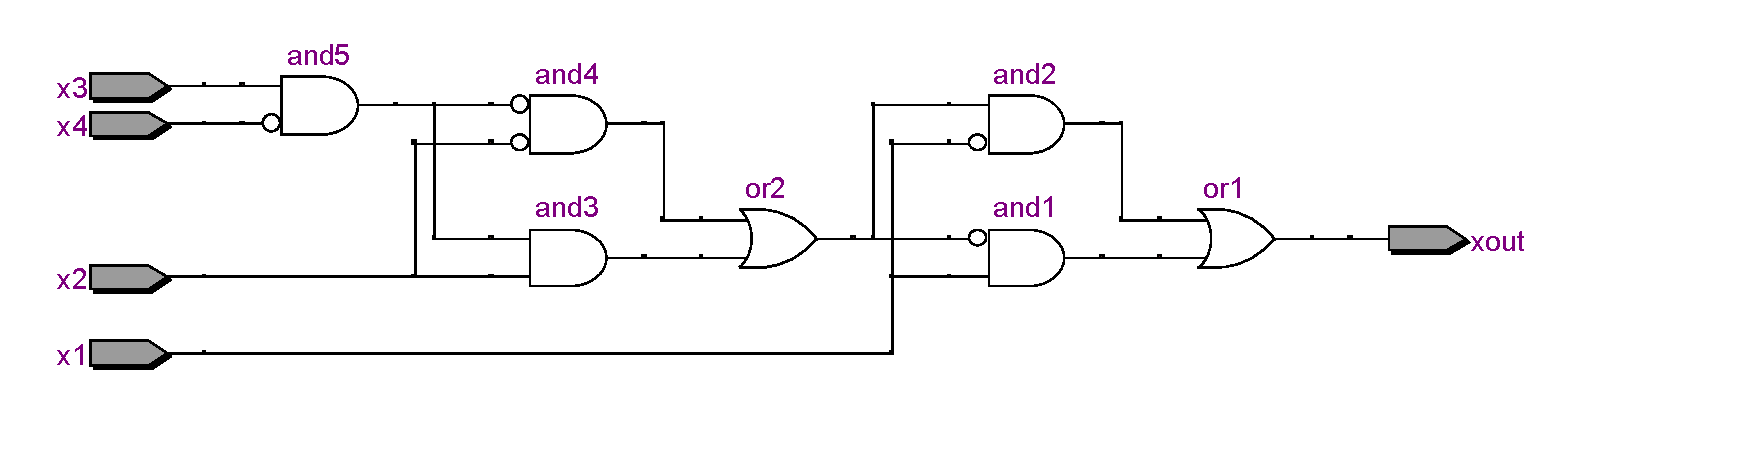
\includegraphics[scale=0.50]{images/ursk.pdf}

Nun stellen wir in unserem neuen Schaltkreis f\"ur jedes Gatter
die Projektion und sein Inverses bereit. Der neue Schaltkreis hat eine Gr\"o\ss{}enkomplexit von 14 also $7 \cdot 2 = 14$ somit erf\"ullt er das Lemma. \\


% Nun stellen wir f\"ur jedes Gatter vom Ende aus auch sein Inverses bereit nach der Regel von deMorgan, bis wir bei
% den Inputs angekommen sind. F\"ur jedes der Inputs stellen wir nun auch das Inverse bereit und verkn\"upfen diese mit den Gattern.
% Bei diesem Schritt k\"onnen \"aquivalente Teilschaltkreise entstehen, die wir wieder zusammen fassen k\"onnen, sodass wir eine Komplexit\"at von 14 erreichen.
% Somit erhalten wir den folgenen Schaltkreis.\\

% Dieser Schaltkreis ist um $U_2$ so wie es das Lemma bereits verlangt.
% Es hat eine $C(s) = 7$ dem zu folge sollte der neue Schaltkreis maximal eine von $14$ haben.
% Zu erst stellen wir zu jedem Input auch sein Inverses bereit und von oben nach Unten (top down) stellen wir nun
% f\"ur jedes Gatter auch sein Inverses nach den Regeln von DeMorgan zu verf\"ugung.
% Bei diesem Schritt kann es dazu kommen das wir zwei \"aquivalente Teilschaltkreise bekommen die wir zusammen f\"ugen k\"onnen. \\

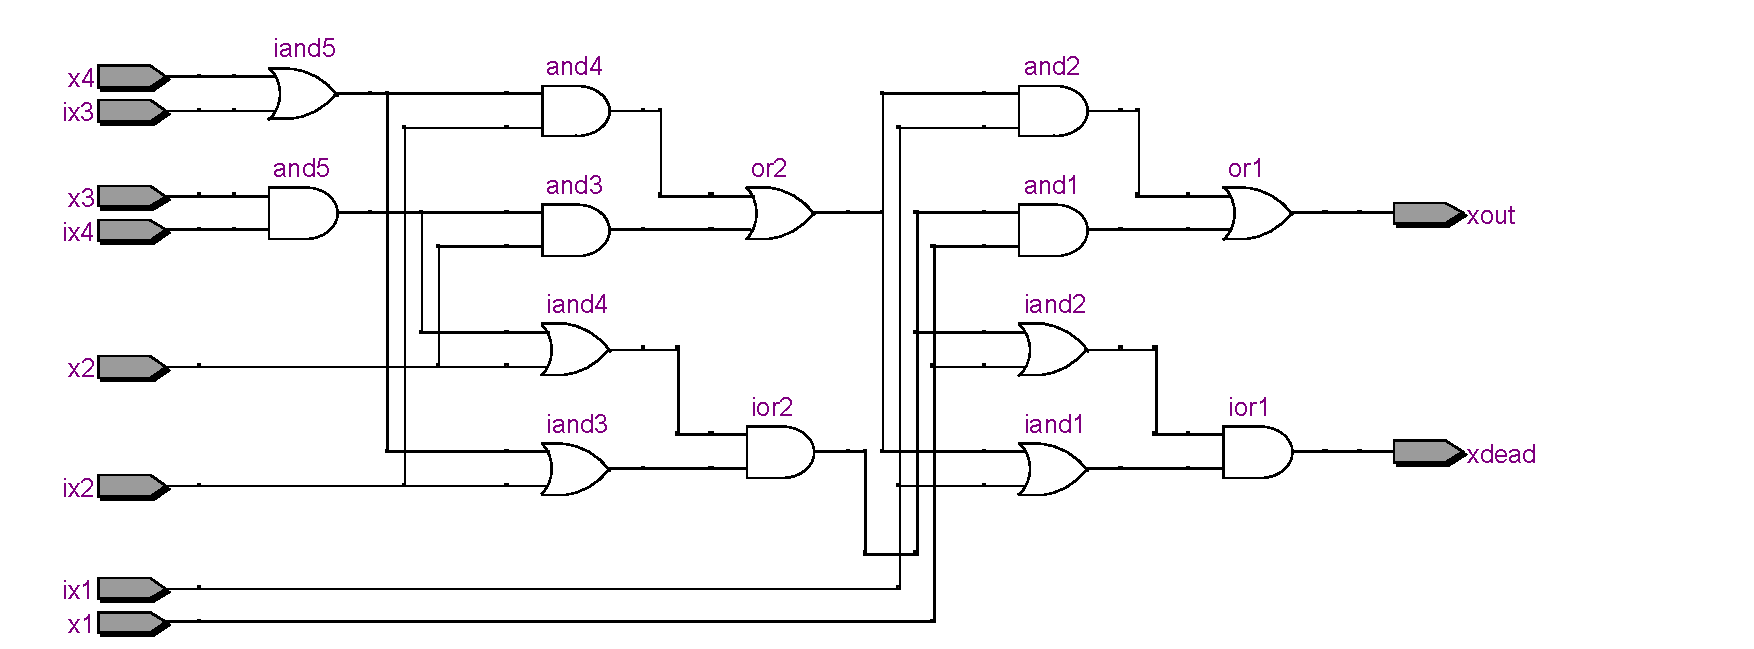
\includegraphics[scale=0.50]{images/zwisk.pdf}

Am Ende entfernen wir noch die f\"ur den Ausgang irrelevanten Gatter erreichen das unser Schaltkreis sogar kleiner
als 14 geworden ist, n\"amlich 11.\\

% Jetzt k\"onnen wir alle \glqq toten\textquotedblright $\;$Gatter entfernen um den Schaltkreis zu optimieren und erreichen eine Komplexit\"at von 11.\\

% Dieser neue Schaltkreis hat nun eine Komplexit\"at von $14$, also h\"alt er sich an das Lemma. Die Not-Gatter sind auch alle verschwunden und werden nun \"uber
% die Inversen Inputs realisiert. Zum Schluss k\"onnen wir noch \glqq M\"ull\grqq entfernen. Also tote Gatter die wir nicht ben\"otigen da ihre Signale ins Nirvana verschwinden.\\

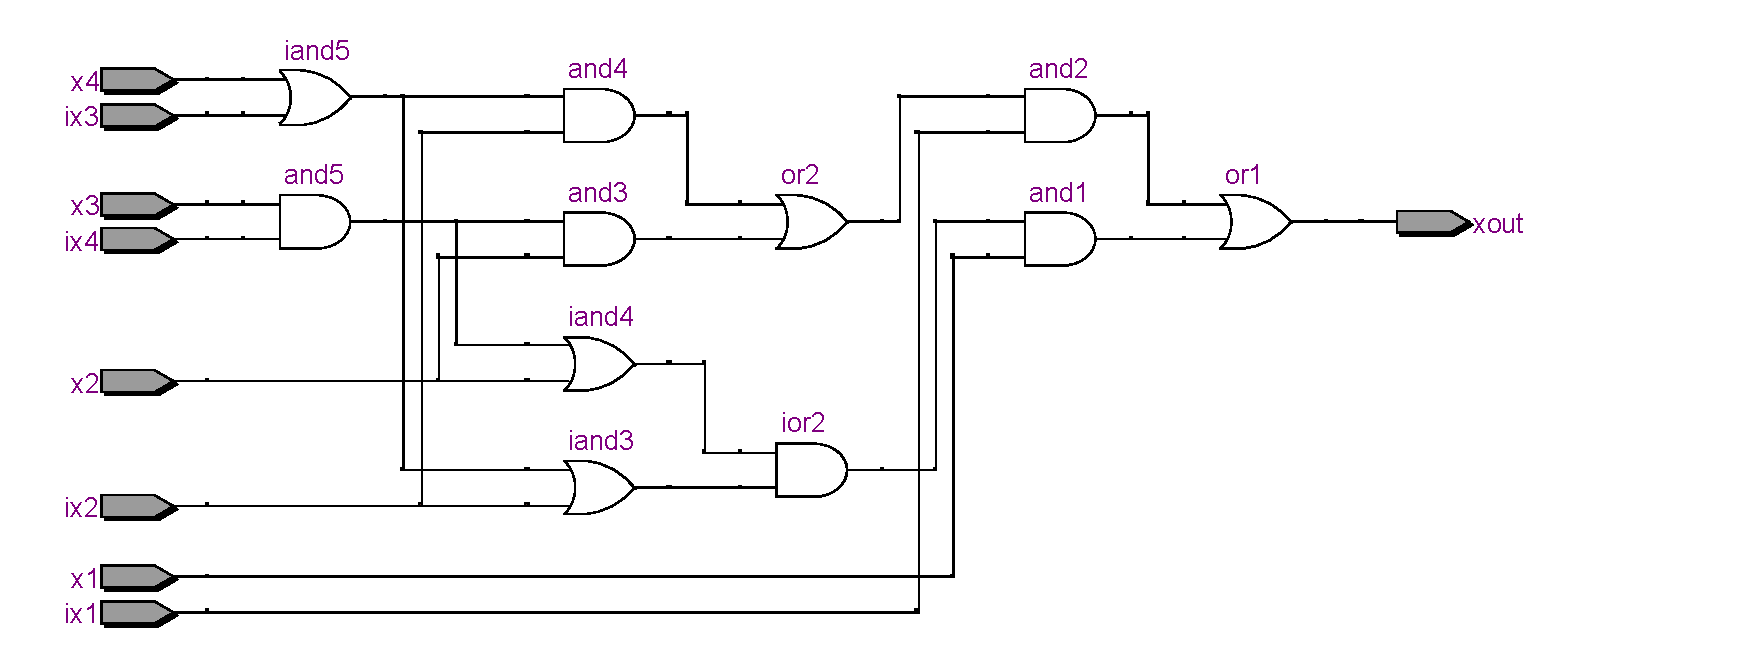
\includegraphics[scale=0.50]{images/endsk.pdf}

% Am Ende konnten wir wieder 3 Gatter entfernen und konnten somit den Schaltkreis optimieren. Die neue Komplexit\"at ist nun $11$ und damit ist diese geringer als das Zweifache der Komplexit\"at des Urschaltkreises.


\end{document}